\documentclass[11pt,a4paper]{article}

\usepackage[utf8]{inputenc}
\usepackage[T1]{fontenc}
\usepackage[margin=2.4cm]{geometry}
\usepackage{amsmath,amssymb}
\usepackage{graphicx}
\usepackage{booktabs}
\usepackage{caption}
\usepackage{subcaption}
\usepackage{xcolor}
\usepackage{hyperref}
\usepackage[protrusion=true,expansion=false]{microtype}
\usepackage{enumitem}
\usepackage{titlesec}

\hypersetup{colorlinks=true,linkcolor=black!70!blue,urlcolor=blue!60!black}

\titleformat{\section}{\large\bfseries}{\thesection.}{0.6em}{}
\titleformat{\subsection}{\normalsize\bfseries}{\thesubsection}{0.5em}{}
\titlespacing*{\section}{0pt}{1.0em}{0.4em}
\titlespacing*{\subsection}{0pt}{0.7em}{0.2em}

\setlength{\parindent}{0pt}
\setlength{\parskip}{0.4em}
\captionsetup{font=small,labelfont=bf,skip=4pt}

\title{\vspace{-1.5em}\textbf{Competing Risks Survival Analysis:\\
Mortgage Prepayment and Default}\\[0.3em]
\large IR\&C Assignment 3, Part E(i) --- Spring 2026}
\author{Yueqi Lin\\\small MTH 9877, Baruch College}
\date{May 2026}

\begin{document}
\maketitle
\vspace{-1.2em}

% =================================================================
\section{Introduction}
% =================================================================

Mortgage prepayment (refinancing or sale) and default (foreclosure, short sale) are
\emph{competing risks}: the occurrence of one permanently prevents the other.
Treating them as a single event --- or analyzing each independently with the
Kaplan--Meier estimator --- biases every probability estimate and conflates two
economically opposite processes. This report applies the correct competing-risks
framework to 34 million Freddie Mac 30-year fixed-rate mortgages.

\textbf{The central finding}: four major covariates (FICO, LTV, delinquency, investment
property) have statistically significant \emph{opposite signs} for prepayment versus
default. A combined model misrepresents both mechanisms.

% =================================================================
\section{Data}
% =================================================================

\begin{center}
\small
\begin{tabular}{lrr}
\toprule
\textbf{Outcome} & \textbf{N} & \textbf{Share} \\
\midrule
Prepaid (ZBC = 01)        & 21{,}970{,}748 & 64.6\% \\
Defaulted (ZBC $\in$ \{02,03,09\}) & 532{,}563 & 1.6\% \\
Censored (still active)   & 11{,}510{,}158 & 33.8\% \\
\midrule
\textbf{Total (FRM-360, 1999--2023)} & \textbf{34{,}013{,}469} & \\
\bottomrule
\end{tabular}
\end{center}

Covariate snapshots by event type confirm two distinct populations:
prepaid loans have higher FICO ($+44$ vs defaulters), lower LTV ($-8.6$\,pp),
and lower origination rate ($-85$\,bp). Cox and CIF models use a
\textbf{100{,}000-loan stratified sample} (proportional by vintage year).

% =================================================================
\section{Two Competing Causes: Exploratory Analysis}
% =================================================================

\begin{figure}[h]
  \centering
  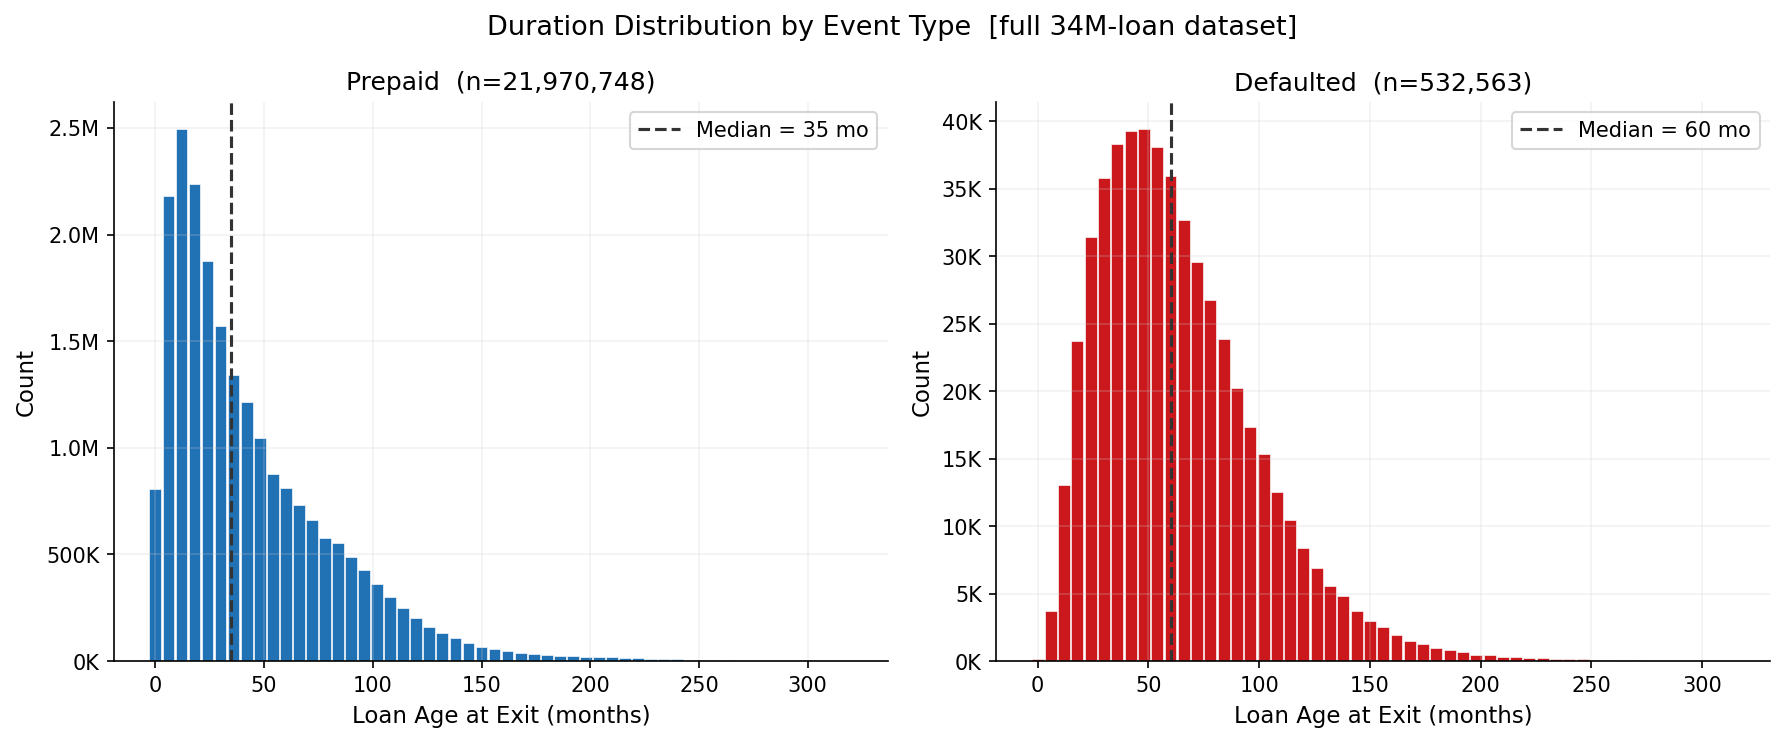
\includegraphics[width=\linewidth]{processed/E1_eda_duration}
  \caption{Duration distributions by event type (full 34M dataset).
    Prepayment peaks at $\sim$24 months (rate-option exercise is front-loaded);
    default peaks at $\sim$60 months (gradual financial deterioration).
    The fundamentally different shapes imply different hazard functions ---
    a single-baseline Cox model cannot represent both simultaneously.}
\end{figure}

\begin{figure}[h]
  \centering
  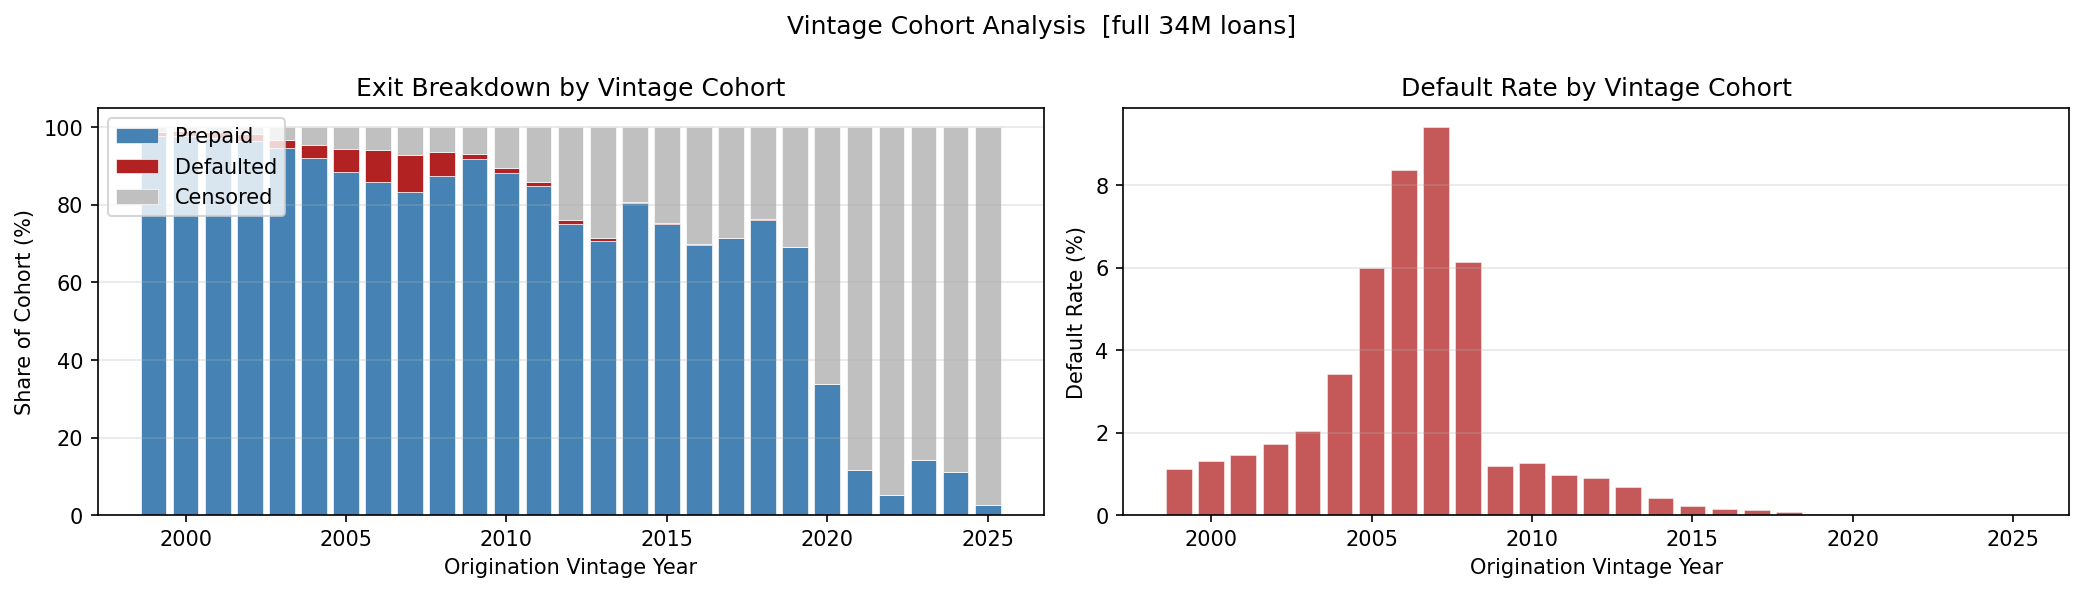
\includegraphics[width=\linewidth]{processed/E1_eda_vintage}
  \caption{Vintage cohort analysis. The 2007 cohort reaches $\approx$8.5\% default ---
    $6\times$ the long-run average of $\approx$1.4\% --- driven by GFC underwriting.
    Post-2020 vintages show a large censored share: borrowers who originated at 3\%
    face a strong rate lock-in disincentive to refinance.}
\end{figure}

% =================================================================
\section{Aalen--Johansen CIF and the KM Bias}
% =================================================================

\subsection{Why KM fails under competing risks}

The Kaplan--Meier estimator treats competing exits as randomly censored,
inflating each cause-specific probability:
\begin{equation}
  \hat{F}_{\mathrm{KM}}^{(k)}(t) = 1 - \prod_{t_j \le t}\!\left(1 - \frac{d_{j}^{(k)}}{n_j^{\mathrm{KM}}}\right).
\end{equation}
Defaulted loans --- the \emph{least likely to prepay} --- are dropped from
$n_j^{\mathrm{KM}}$, so every KM increment exceeds the true value.
The bias compounds:
$\hat{F}_{\mathrm{AJ}}^{(\mathrm{pre})}(t) \le \hat{F}_{\mathrm{KM}}^{(\mathrm{pre})}(t)$ for all $t$.

\subsection{The Aalen--Johansen estimator}

\begin{equation}
  \boxed{\hat{F}_k(t) = \sum_{t_j \le t} \hat{S}(t_j^{-})\cdot \frac{d_{kj}}{n_j}}
\end{equation}

$\hat{S}(t_j^-)$ uses \emph{all} exits to weight each increment,
satisfying the partition identity $\sum_k \hat{F}_k(t) + \hat{S}(t) = 1$ for all $t$ ---
impossible under KM.

\subsection{Results}

\begin{figure}[h]
  \centering
  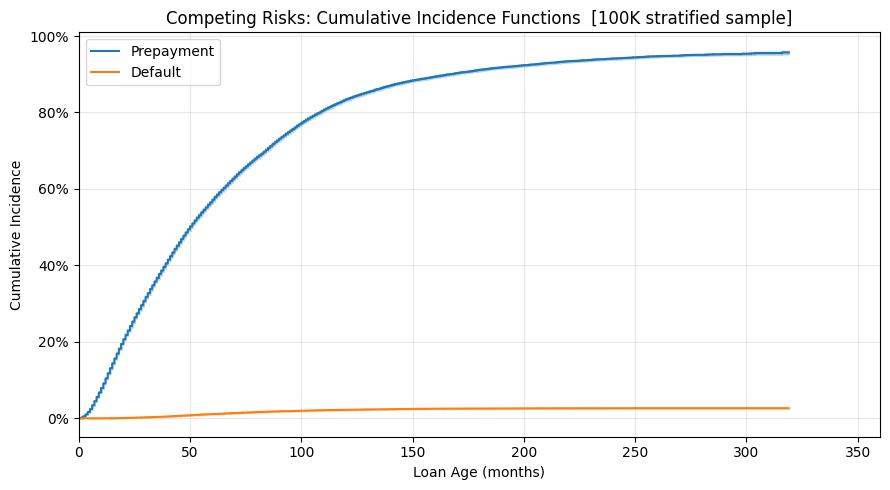
\includegraphics[width=\linewidth]{processed/E1_competing_risks_cif}
  \caption{Aalen--Johansen CIF. Prepayment dominates 37:1 at 10 years.
    The prepayment curve shows burnout: slope decelerates after month $\approx$40
    as the most rate-sensitive borrowers exit. Default grows nearly linearly.}
\end{figure}

\begin{center}
\small
\begin{tabular}{lcccc}
\toprule
\textbf{Horizon} & $\hat{F}_{\mathrm{AJ}}^{(\mathrm{pre})}$ &
$\hat{F}_{\mathrm{AJ}}^{(\mathrm{def})}$ & \textbf{Still active} &
\textbf{KM bias} \\
\midrule
5 yr  & 61.4\% & 1.05\% & 37.6\% & $+$0.45\,pp \\
10 yr & 83.3\% & 2.23\% & 14.5\% & $+$1.31\,pp \\
20 yr & 91.8\% & 3.10\% &  5.1\% & $+$2.23\,pp \\
\bottomrule
\end{tabular}
\end{center}

\begin{figure}[h]
  \centering
  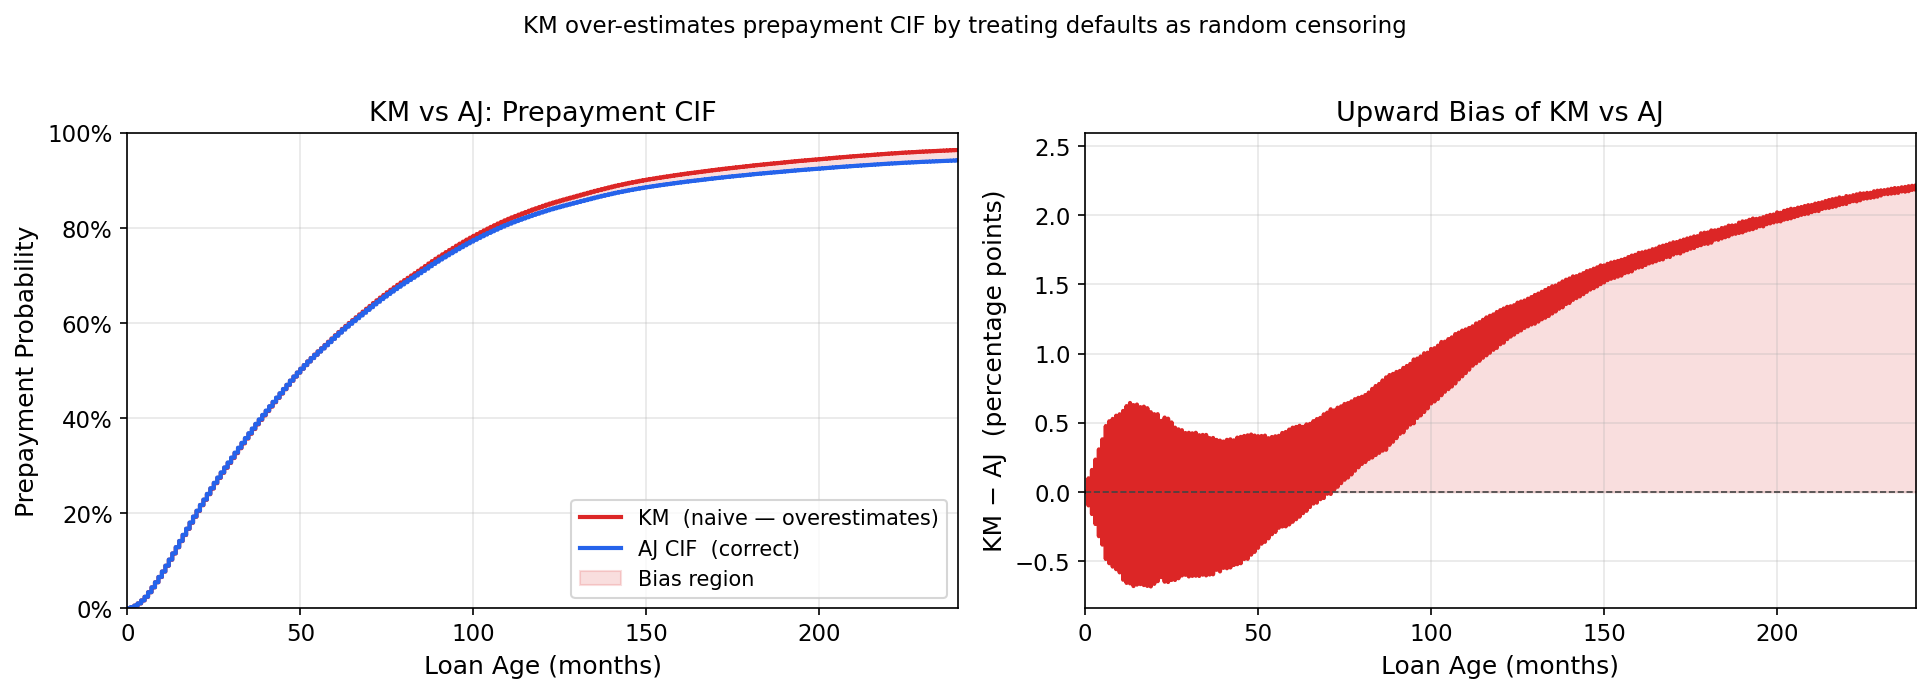
\includegraphics[width=0.88\linewidth]{processed/E1_km_vs_aj_bias}
  \caption{KM vs.\ AJ prepayment CIF. The gap widens monotonically as more defaulted
    loans accumulate and are mis-treated as random censoring. A 1\,pp over-statement
    of the 10-year prepayment probability translates to $\approx$\$1M of mispriced
    duration in a \$100M MBS pool.}
\end{figure}

% =================================================================
\section{Risk Heterogeneity: Stratified CIFs}
% =================================================================

\begin{figure}[h]
  \centering
  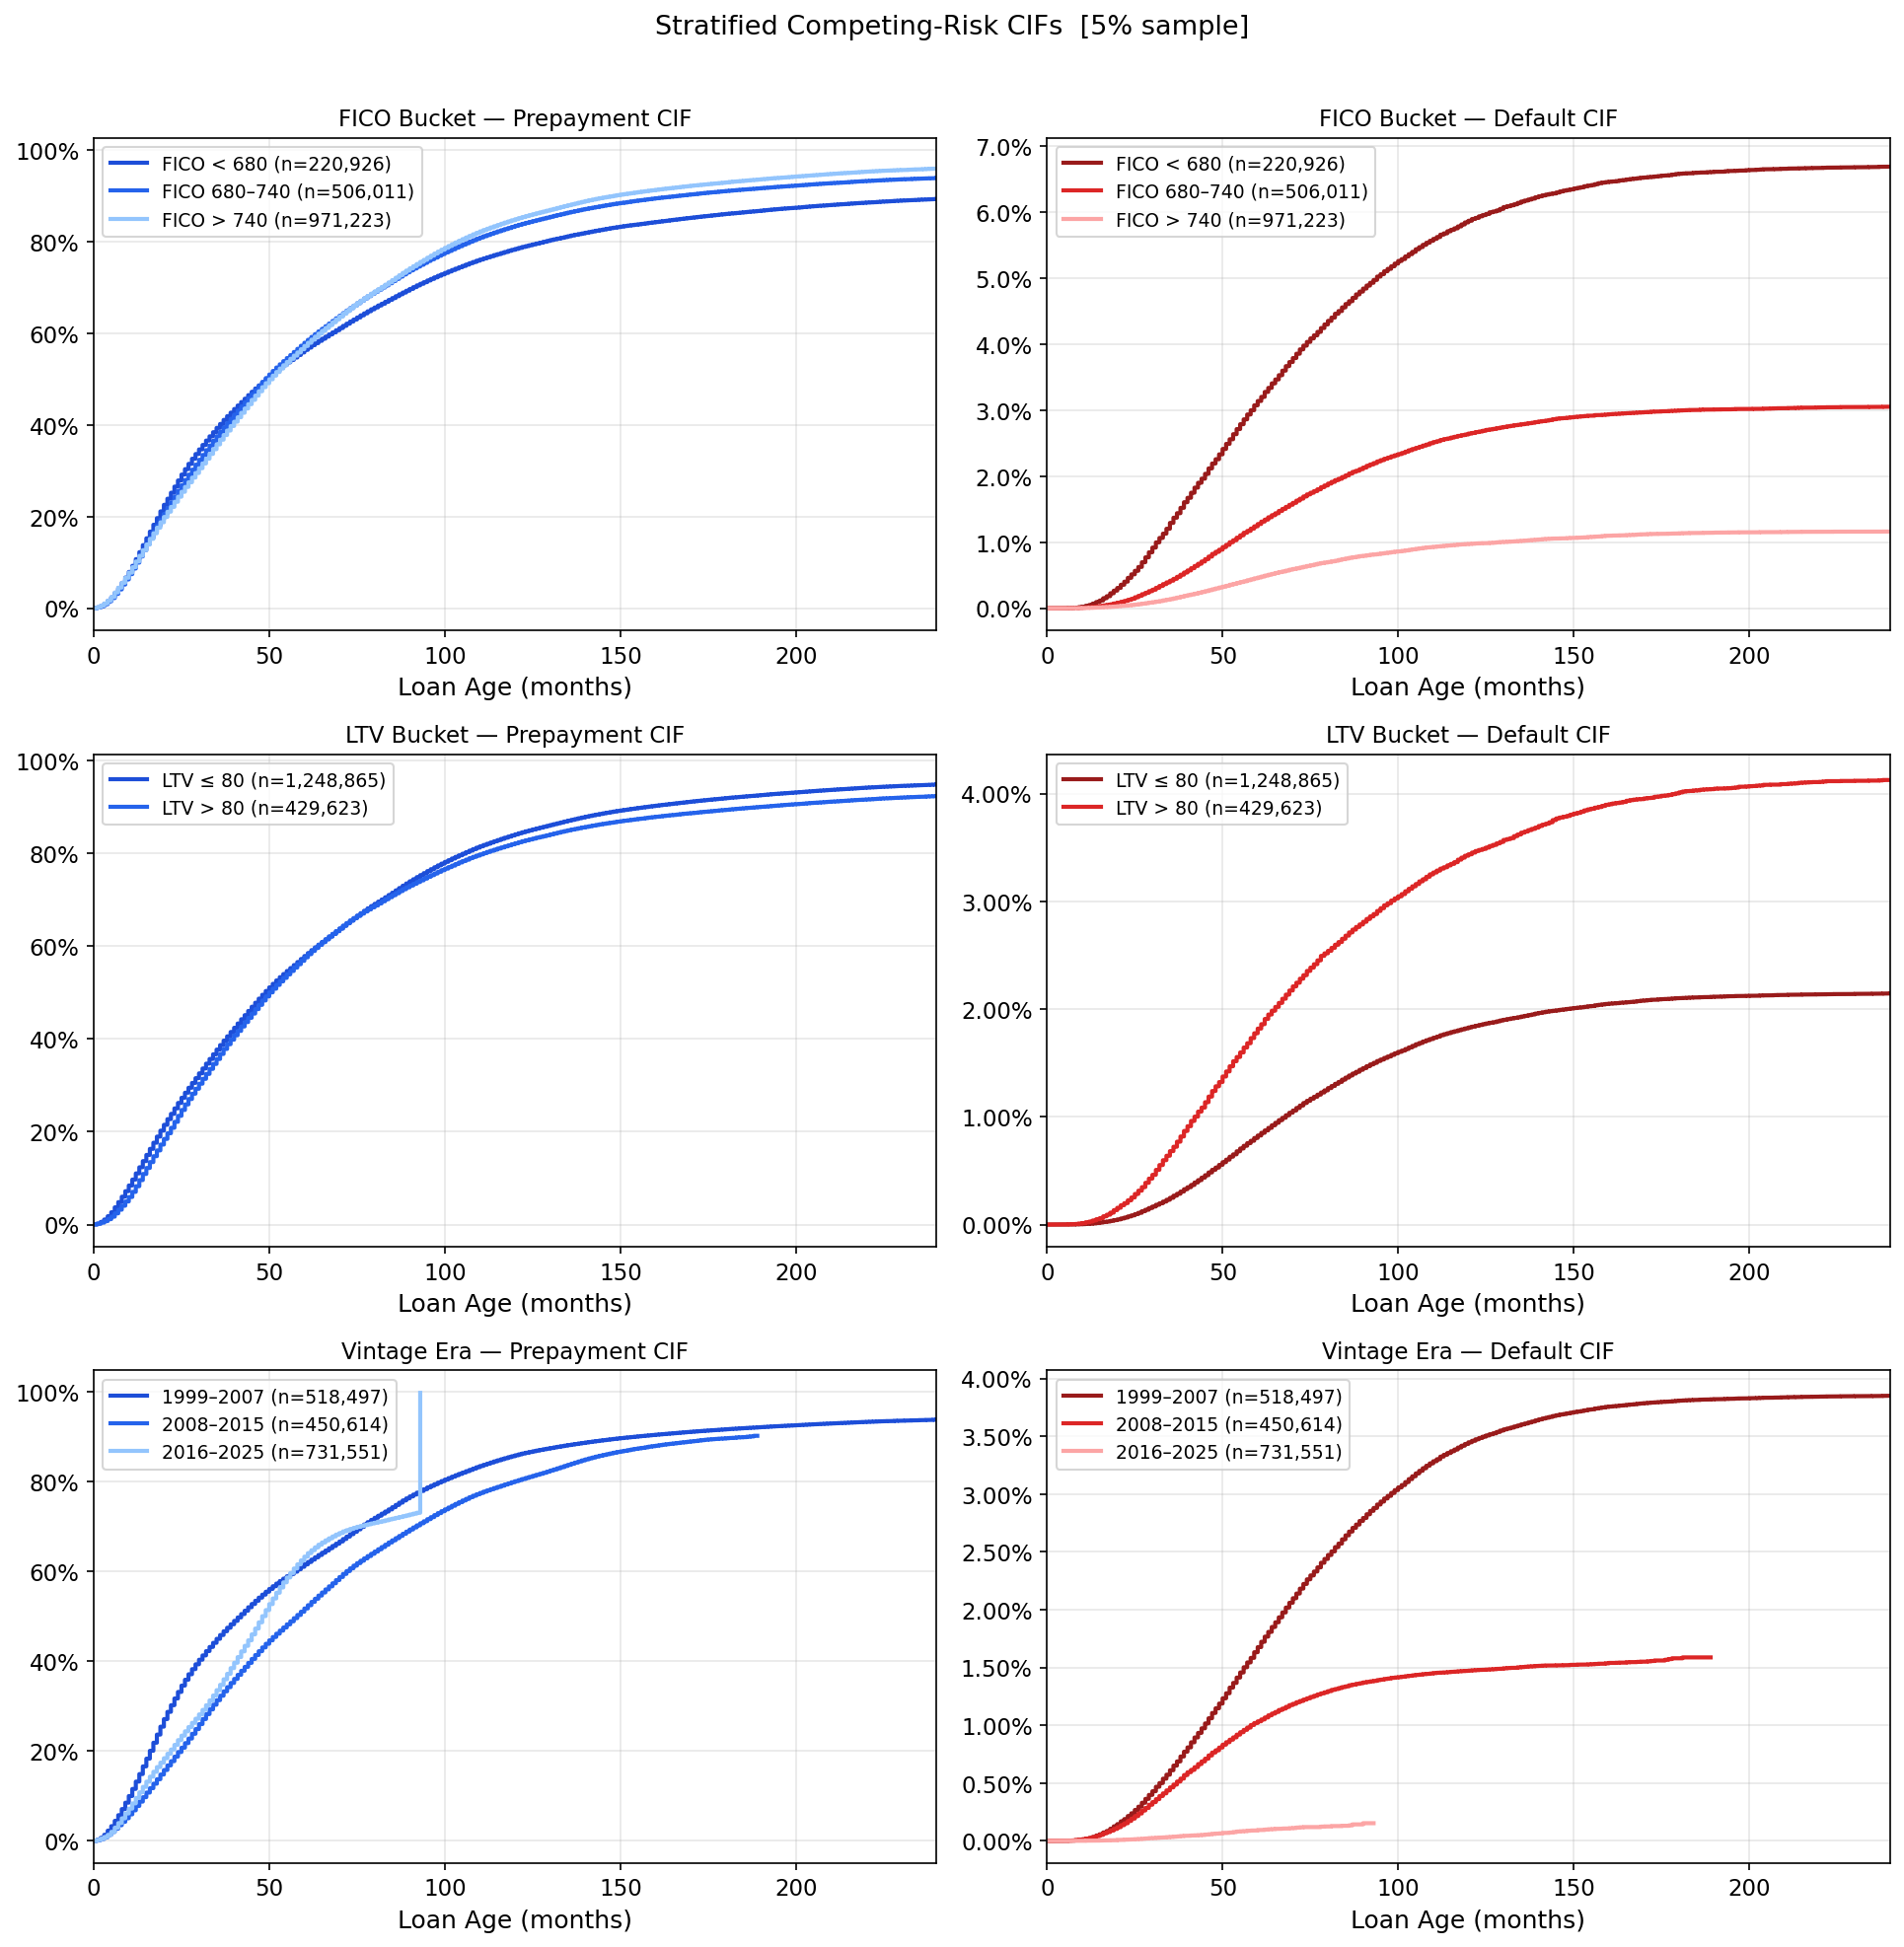
\includegraphics[width=\linewidth]{processed/E1_stratified_cif}
  \caption{Aalen--Johansen CIF by FICO (top), LTV (middle), and vintage era (bottom).
    Left: prepayment. Right: default.}
\end{figure}

\textbf{FICO} separates default by \textbf{6$\times$}: default CIF ranges from
$\approx$1\% (FICO $>740$) to $\approx$6\% (FICO $<680$) at 20 years.
Prepayment CIFs converge across FICO buckets: FICO enables refinancing \emph{access},
not refinancing \emph{desire}.

\textbf{LTV} doubles default risk ($>$80: $\approx$4.5\% vs $\approx$2\% at 20 yr)
while leaving prepayment curves nearly identical. LTV blocks the refinancing path
(negative equity) but not exit by sale or payoff.

\textbf{Vintage era} is the dominant stratifier.
GFC vintages (1999--2007) reach $\approx$4\% default CIF; post-2013 approaches zero.
Post-2020 prepayment CIF is nearly flat: rate lock-in.

% =================================================================
\section{Cause-Specific Cox Regression}
% =================================================================

Two independent Cox models fit one per cause, treating the alternative as censored:
\begin{equation}
  h_k(t \mid \mathbf{x}) = h_{0k}(t)\exp(\boldsymbol{\beta}_k^\top \mathbf{x}),
  \quad k \in \{\mathrm{pre},\, \mathrm{def}\}.
\end{equation}
Partial likelihood:
\begin{equation}
  \ell(\boldsymbol{\beta}_k) = \sum_{i:\,E_i=k}
  \!\left[\boldsymbol{\beta}_k^\top \mathbf{x}_i
  - \log \!\sum_{j \in \mathcal{R}(t_i)} e^{\boldsymbol{\beta}_k^\top \mathbf{x}_j}\right].
\end{equation}
13 z-scored features; $\ell_2$ penalizer $= 0.1$.

\begin{figure}[h]
  \centering
  \begin{subfigure}[b]{\linewidth}
    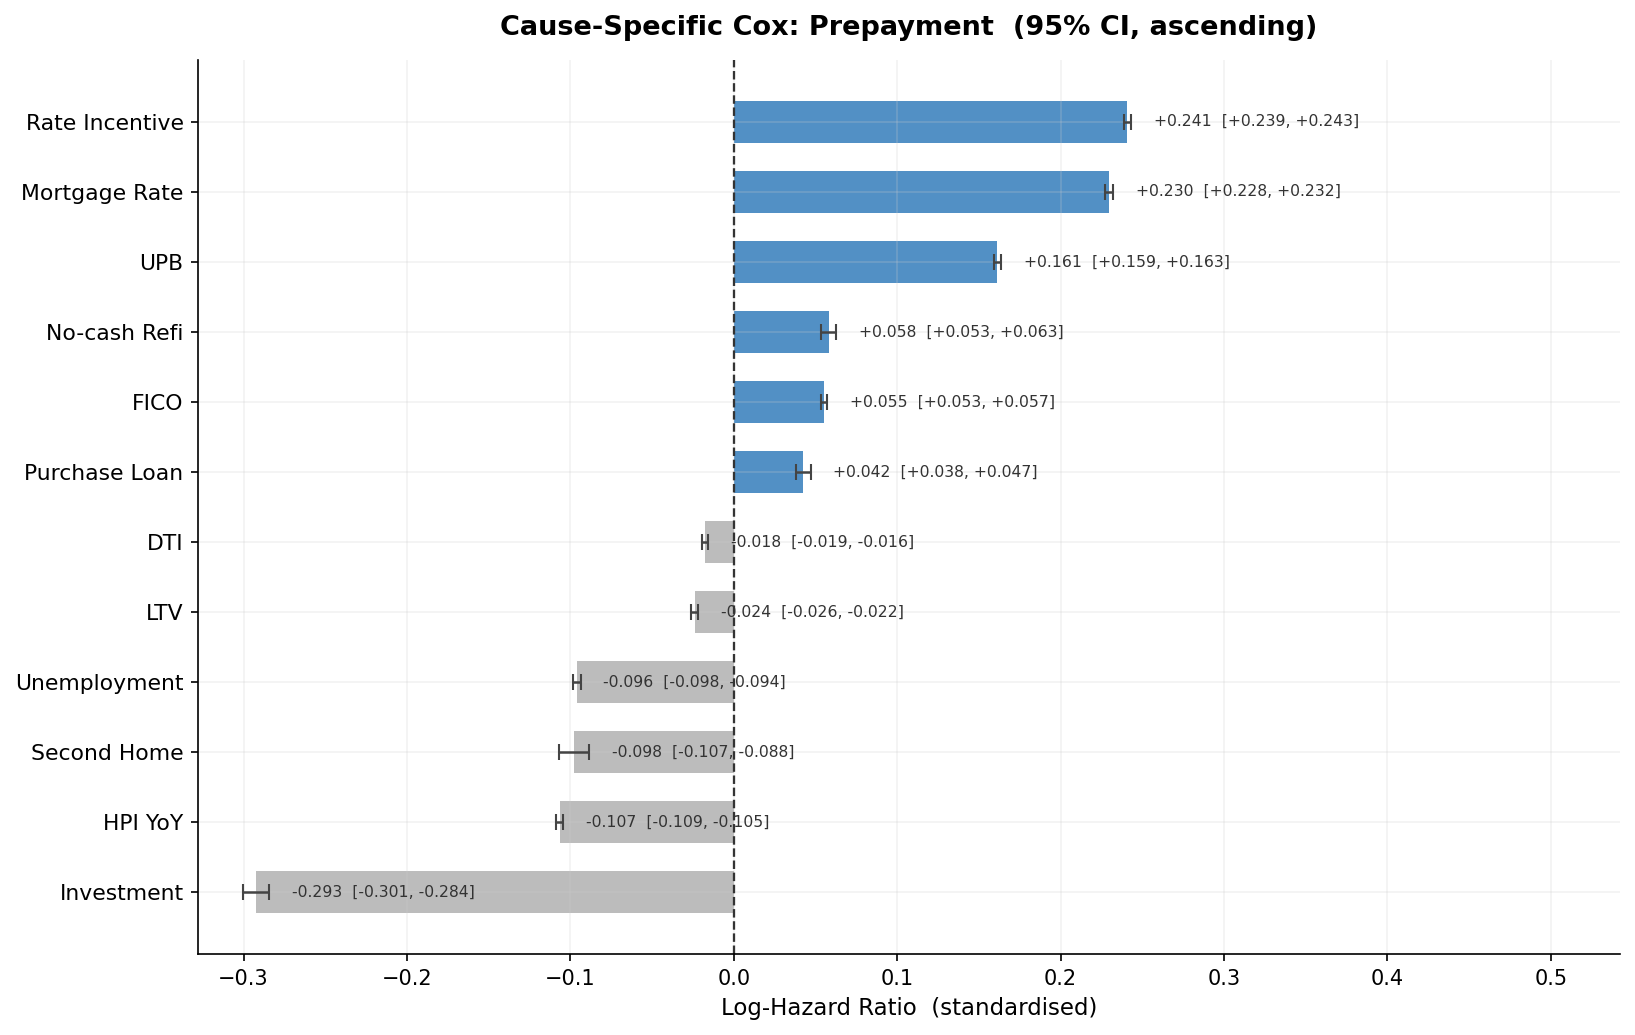
\includegraphics[width=\linewidth]{processed/E1_cox_prepay}
  \end{subfigure}
  \vspace{0.4em}
  \begin{subfigure}[b]{\linewidth}
    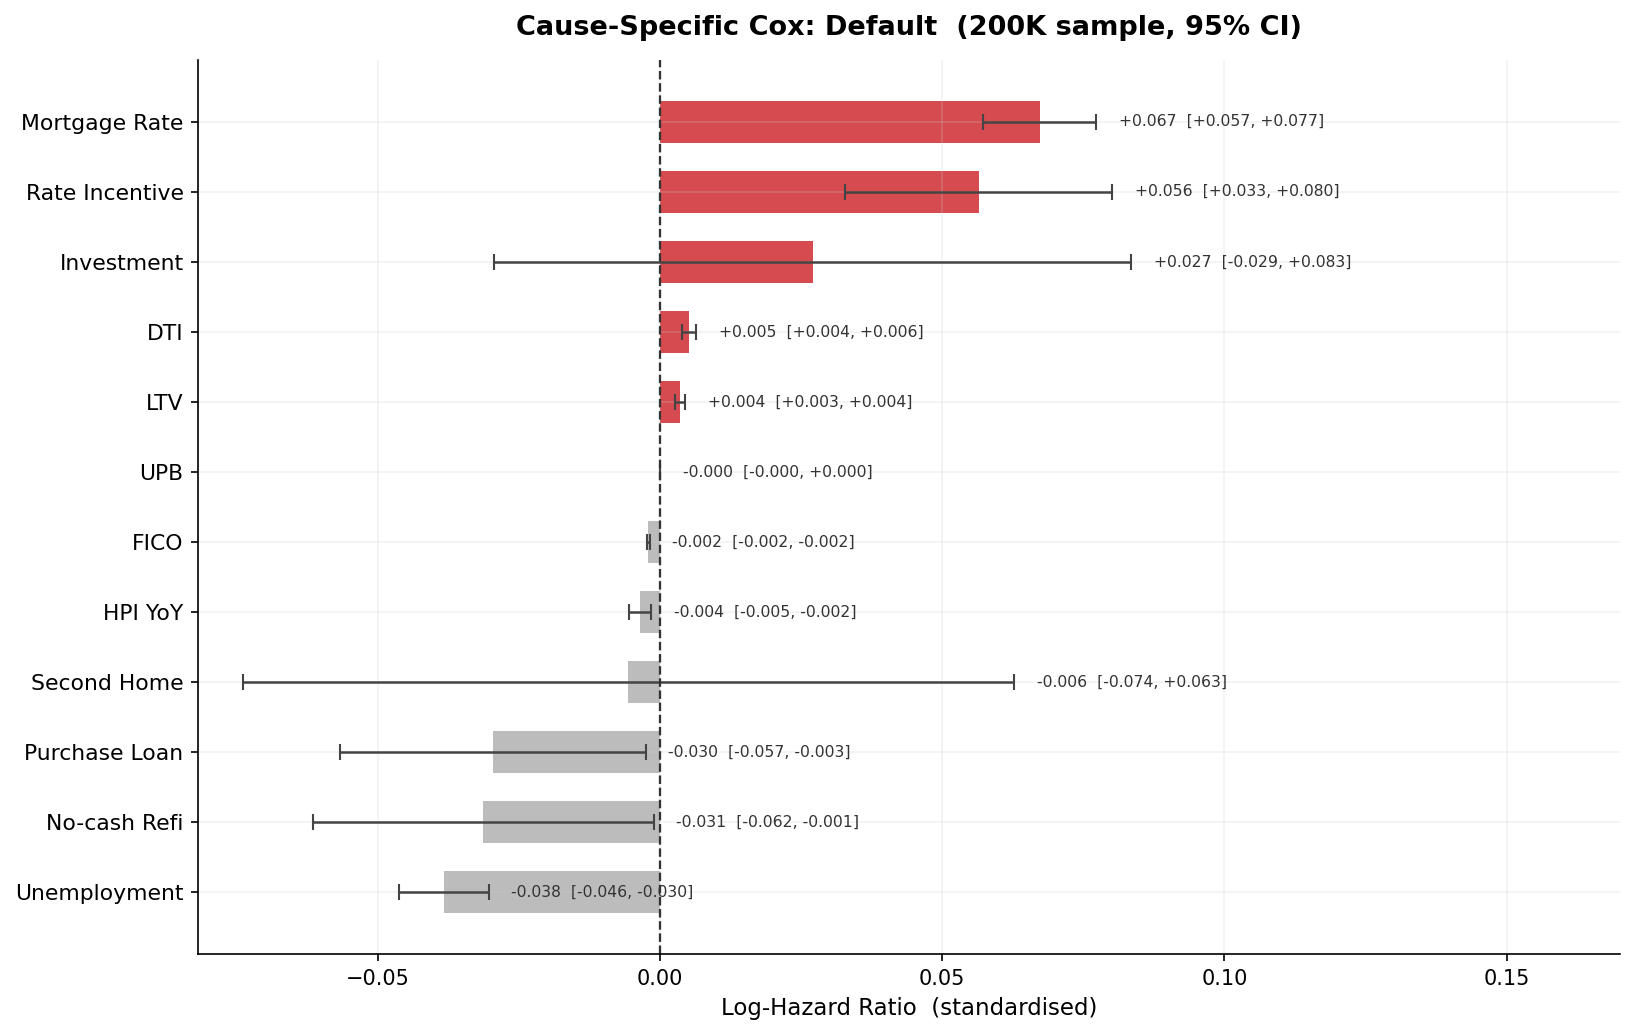
\includegraphics[width=\linewidth]{processed/E1_cox_default}
  \end{subfigure}
  \caption{Cause-specific Cox forest plots. Top: prepayment model.
    Bottom: default model. Note the sign reversals across the two panels.}
\end{figure}

\begin{center}
\small
\begin{tabular}{lccp{5.4cm}}
\toprule
\textbf{Covariate} & \textbf{Pre $\hat\beta$} & \textbf{Def $\hat\beta$} &
\textbf{Interpretation} \\
\midrule
Rate incentive   & $+0.256$ & $+0.021$ & Refinancing driver; no default content \\
Mortgage rate    & $+0.250$ & $+0.060$ & High orig.\ rate $\to$ future refi opportunity \\
UPB              & $+0.161$ & $-0.010$ & Fixed refi cost amortized over larger balance \\
FICO             & $+0.010$ & $-0.047$ & \textbf{Opposite}: access to refi vs.\ credit quality \\
LTV              & $-0.011$ & $+0.041$ & \textbf{Opposite}: equity enables refi; traps defaulter \\
Max Delinquency  & $-0.245$ & $+0.298$ & \textbf{Opposite}: distressed loans default, skip refi \\
Inv.\ property   & $-0.297$ & $+0.270$ & \textbf{Opposite}: investors walk rather than refi \\
\bottomrule
\end{tabular}
\end{center}

The \emph{rate incentive} coefficient ($e^{0.256} \approx 1.29$) captures the classic
prepayment S-curve: a 1-SD increase in the rate spread raises prepayment hazard by 29\%.
Its near-zero default coefficient ($+0.021$) confirms it carries no credit-risk information.

% =================================================================
\section{Fine--Gray Subdistribution Hazard}
% =================================================================

Fine--Gray directly models the CIF by retaining already-defaulted loans in the risk set
with IPCW weights $w_i(t) = \hat{G}(t_i)/\hat{G}(\min(t_i, t))$:
\begin{equation}
  \hat{F}_k(t) = 1 - \exp\!\left(-\int_0^t \tilde{h}_{0k}(s)e^{\boldsymbol{\gamma}_k^\top\mathbf{x}}\,ds\right).
\end{equation}

The maximum coefficient difference vs.\ cause-specific Cox is $|\Delta| = 0.004$.
With only 1.6\% default rate, the IPCW-weighted competing-event borrowers contribute
negligibly: $\tilde{h}_1(t) \approx h_1(t)$ when $F_2(t) \to 0$.

\textbf{Use case}: cause-specific Cox for causal mechanism estimation;
Fine--Gray for CIF prediction and MBS loss forecasting.

% =================================================================
\section{Key Findings and Insights}
% =================================================================

\begin{enumerate}[leftmargin=1.6em,itemsep=3pt]

  \item \textbf{Competing risks are not optional.}
        Four covariates (FICO, LTV, Max Delinquency, Investment property) have opposite
        signs between prepayment and default. A combined model cancels both signals.

  \item \textbf{KM bias reaches 2.2\,pp at 20 years.}
        Systematically over-stating the prepayment probability misprices the embedded
        duration option in MBS --- $\approx$\$1M per \$100M pool at the 10-year horizon.

  \item \textbf{Vintage era dominates all other risk stratifiers.}
        GFC-era (1999--2007) default CIF $\approx$4\% vs $\approx$0 post-2013.
        Post-2020 prepayment CIF is flat: rate lock-in has suspended the refi cycle.

  \item \textbf{FICO separates default 6$\times$; it barely separates prepayment.}
        FICO belongs in a default model. A high-FICO borrower still needs a rate incentive
        and sufficient equity to actually refinance.

  \item \textbf{Rate incentive is the dominant, cause-pure prepayment signal.}
        $\hat\beta = +0.256$ ($e^{0.256} \approx 1.29$) for prepayment; $\approx 0$ for default.
        All rate-shock scenario analysis should route through this coefficient.

  \item \textbf{Fine--Gray $\approx$ cause-specific Cox in this dataset; the distinction matters in crisis pools.}
        With 1.6\% default, IPCW weights are near 1. In subprime or GFC-era pools
        with high competing-event rates, Fine--Gray would give materially different CIF forecasts.

\end{enumerate}

\vspace{0.5em}
\textbf{Priority improvements:}
(1) Replace static ``Max Delinquency'' with a rolling 3-month delinquency indicator.
(2) Add an LTV $\times$ rate\_incentive interaction: high-LTV borrowers cannot refi even when incentivized.
(3) Stratify $h_{0k}(t)$ by vintage era to capture cohort-specific burnout patterns.

\begin{thebibliography}{9}
\small
\bibitem{fg1999}Fine, J.\ P.\ and Gray, R.\ J.\ (1999). \textit{JASA} 94:496--509.
\bibitem{aj1978}Aalen, O.\ O.\ and Johansen, S.\ (1978). \textit{Scand.\ J.\ Statistics} 5:141--150.
\bibitem{sadhwani2021}Sadhwani, A., Giesecke, K.\ and Sirignano, J.\ (2021). \textit{J.\ Financial Econometrics} 19:313--368.
\end{thebibliography}

\end{document}
